\documentclass{article}
\usepackage{graphicx} % Required for inserting images
\usepackage[export]{adjustbox}% Required for inserting images
\usepackage{float}
\usepackage{placeins}
\title{PS03_myanswers_AG}
\author{Aryan Goyal}
\date{October 2023}

\begin{document}
\section{PS03 Answers}
Aryan Goyal

\noindent Student number: 18306046
\vspace{0.2cm}

\noindent First, I import the data into R
\begin{verbatim}
    incumbent <- read.csv("https://raw.githubusercontent.com/ASDS-TCD/StatsI_Fall2023/main/datasets/incumbents_subset.csv")
\end{verbatim}

\section{Question 1}
    
\subsection{Answer 1a)}
I run a linear regression using the lm function where the outcome variable is voteshare and the explanatory variable is difflog
\begin{verbatim}
    q1 <- lm(voteshare~difflog, data=incumbent)
    summary(q1)

\end{verbatim}

\begin{table}[!htbp] \centering 
  \caption{Bivariate Regression between difflog(X) and vote share (Y)} 
  \label{} 
\begin{tabular}{@{\extracolsep{5pt}}lc} 
\\[-1.8ex]\hline 
\hline \\[-1.8ex] 
 & \multicolumn{1}{c}{\textit{Dependent variable:}} \\ 
\cline{2-2} 
\\[-1.8ex] & Vote share \\ 
\hline \\[-1.8ex] 
  Constant & 0.579$^{***}$ \\ 
  & (0.002) \\ 
  & \\ 
  Difflog & 0.042$^{***}$ \\ 
  & (0.001) \\ 
  & \\ 
\hline \\[-1.8ex] 
Observations & 3,193 \\ 
R$^{2}$ & 0.367 \\ 
Adjusted R$^{2}$ & 0.367 \\ 
Residual Std. Error & 0.079 (df = 3191) \\ 
F Statistic & 1,852.791$^{***}$ (df = 1; 3191) \\ 
\hline 
\hline \\[-1.8ex] 
\textit{Note:}  & \multicolumn{1}{r}{$^{*}$p$<$0.1; $^{**}$p$<$0.05; $^{***}$p$<$0.01} \\ 
\end{tabular} 
\end{table} 
 
\vspace{0.3cm}

\noindent Our null hypothesis is that there is no association between difference in campaign spending (X) and the incumbent's vote share (Y), $\beta_1 = 0$. $\beta_1$ represents the slope or the regression coefficient of the explanatory variable

The alternative hypothesis is that there is an association between difference in campaign spending (X) and the incumbent's vote share (Y), $\beta_1 \neq 0$.

As shown in Table 1, $\beta_1$ is significant at the 0.01 alpha level, hence we can reject the null hypothesis and we find support for the alternative hypothesis that there is an association between difference in campaign spending and incumbent's vote share, $\beta_1 \neq 0$. 
Moreover, we can say that for a 1 unit increase in difference in campaign spending (X), there is 0.042 scale points increase in incumbent's vote share(Y).

\noindent I am not interpreting the $\beta_0$ value as it does not make sense in this context. If the difference in campaign spending (X) = 0, the incumbent's vote share (Y) = 0.579 scale points which does not provide us with any relevant understanding.

\subsection{Answer 1b)}
I make a scatterplot with both variables along with a regression line.
I also add the correlation value to understand the strength and direction of the linear relationship.
\begin{verbatim}
    plot(incumbent$difflog, incumbent$voteshare, main='Relationship between incumbent 
    voteshare and difference in campaign spending',
    xlab='Difference in campaign spending',ylab='Vote Share')
abline(lm(voteshare~difflog, data=incumbent),col='red',lty='dashed') 
cor(incumbent$voteshare,incumbent$difflog)
text(-2, 0.9,sprintf("Correlation=%s",
round(cor(incumbent$difflog,incumbent$voteshare),4)))
\end{verbatim}

\begin{figure}[h!] %%Code to put figures in the pdf
    \centering
    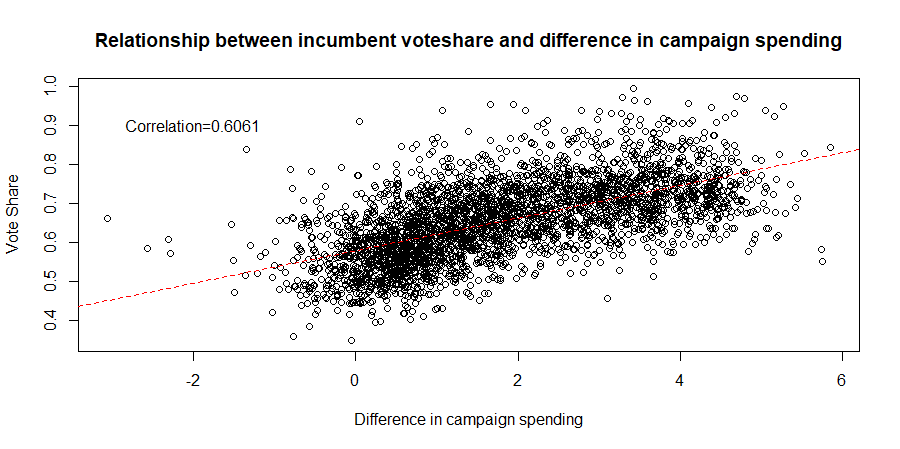
\includegraphics[width=1.3\textwidth]{Q1PS3.png}
    \caption{Relationship between Incumbent Vote Share and difference in 
    Campaign Spending}
    \label{}
\end{figure}

On the basis of the regression line and correlation value in Figure 1, we can see a positive strong correlation (0.6061) between difference in campaign spending and the vote share. 

\subsection{Answer 1c)}
I save the residuals of the model in a separate object in R
\begin{verbatim}
    q1residuals <- q1$residuals ##Accessing the residuals using the "$" input
    head(q1residuals)

\end{verbatim}
\subsection{Answer 1d)}
The prediction equation for a simple linear regression can be represented as:
\begin{math} \hat{Y} = \hat{\beta_0} + \hat{\beta_1} * X  \end{math} 

where:

\noindent $\hat{Y}$ is the predicted value of the outcome variable based on the regression equation

\noindent X is the explanatory variable

\noindent $\hat{\beta_0}$ is the estimated y-intercept or the constant term

\noindent $\hat{\beta_1}$ is the estimated coefficient of the explanatory variable indicating the slope of the line

\noindent The error term, $\epsilon$ is inherent in the statistical model, but is not explicitly included in the prediction equation. The error term accounts for the "noise" (variability) in the data that our model does not capture

\vspace{0.3cm}
\noindent Therefore, the prediction equation for our simple linear regression is:

\begin{math}
    vote share = 0.579 + 0.042 * difflog 
\end{math}
\pagebreak
\section{Question 2}

\subsection{Answer 2a)}
I run a linear regression using the lm function where the outcome variable is presvote and the explanatory variable is difflog

\begin{verbatim}
    q2 <- lm(presvote~difflog, data=incumbent)
    summary(q2)
\end{verbatim}

\noindent Our null hypothesis is that there is no association between difference in campaign spending (X) and the vote share of the presidential candidate of the incumbent party (Y), $\beta_1 = 0$

The alternative hypothesis is that there is an association between difference in campaign spending (X) and the vote share of the presidential candidate of the incumbent party (Y), $\beta_1 \neq 0$


\begin{table}[!htbp] \centering 
  \caption{Bivariate regression between
  difflog(X) and presvote(Y)} 
  \label{} 
\begin{tabular}{@{\extracolsep{5pt}}lc} 
\\[-1.8ex]\hline 
\hline \\[-1.8ex] 
 & \multicolumn{1}{c}{\textit{Dependent variable:}} \\ 
\cline{2-2} 
\\[-1.8ex] & Presvote \\ 
\hline \\[-1.8ex] 
  Constant & 0.508$^{***}$ \\ 
  & (0.003) \\ 
  & \\ 
  Difflog & 0.024$^{***}$ \\ 
  & (0.001) \\ 
  & \\ 
\hline \\[-1.8ex] 
Observations & 3,193 \\ 
R$^{2}$ & 0.088 \\ 
Adjusted R$^{2}$ & 0.088 \\ 
Residual Std. Error & 0.110 (df = 3191) \\ 
F Statistic & 307.715$^{***}$ (df = 1; 3191) \\ 
\hline 
\hline \\[-1.8ex] 
\textit{Note:}  & \multicolumn{1}{r}{$^{*}$p$<$0.1; $^{**}$p$<$0.05; $^{***}$p$<$0.01} \\ 
\end{tabular} 
\end{table} 

\noindent As shown in Table 2, $\beta_1$ is significant at the 0.01 alpha level, hence we can reject the null hypothesis and we find support for the alternative hypothesis that there is an association between difference in campaign spending and vote share of the presidential candidate of the incumbent party, $\beta_1 \neq 0$. 
Moreover, we can say that for a 1 unit increase in difference in campaign spending (X), there is 0.024 scale points increase in the vote share of the presidential candidate of the incumbent party(Y).

\noindent Similar to Question 1, the $\beta_0$ is not interpreted as it does not provide us with relevant insight in this context.

%%begin{figure} %%Code to put figures in the pdf
    %centering
    %includegraphics[width=1.3\textwidth]{%%This is where I put the .png file}
    %caption{Y and X1}
    %label{fig:enter-label}
%end{figure}
%%Replace the "%" with \ to use

\subsection{Answer 2b)}
I make a scatterplot with both variables along with a regression line and the correlation value:
\begin{verbatim}
    plot(incumbent$difflog,incumbent$presvote, 
     main='Relationship between difference in campaign spending 
     and vote share of the presidential candidate of the incumbent party',
     xlab='Difference in campaign spending',ylab='Vote share of presidential candidate')
abline(q2,col='red',lty='dashed')
cor(incumbent$presvote,incumbent$difflog)
text(-2, 0.9,sprintf("Correlation=%s", round(cor(incumbent$presvote,incumbent$difflog),4)))
\end{verbatim}

\begin{figure}[h!] %%Code to put figures in the pdf
    \centering
    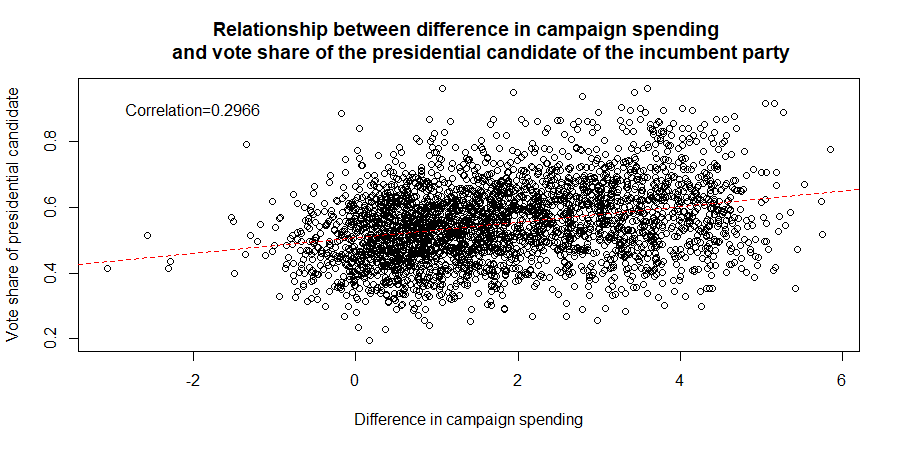
\includegraphics[width=1.3\textwidth]{Q2PS3.png}
    \caption{Relationship between difference in campaign spending 
     and vote share of the presidential candidate of the incumbent party}
    \label{}
\end{figure}

On the basis of the regression line and the correlation value, we can say that there is a weak positive correlation (0.2966) between difference in campaign spending and vote share of presidential candidate of the incumbent party

\subsection{Answer 2c)}
I save the residuals of the model in a separate object in R:
\begin{verbatim}
    q2residuals <- q2$residuals
    head(q2residuals)
\end{verbatim}
\subsection{Answer 2d)}
The prediction equation for our simple linear regression is:

\begin{math}
    Pres Vote = 0.508 + 0.024 * difflog 
\end{math}
\section{Question 3}

\subsection{Answer 3a)}
I run a linear regression using the lm function where the outcome variable is vote share and the explanatory variable is presvote
\begin{verbatim}
    q3 <- lm(voteshare~presvote, data=incumbent)
    summary(q3)
\end{verbatim}

Our null hypothesis is that there is no association between the vote share of the presidential candidate of the incumbent party (X) and the incumbent's vote share (Y), $\beta_1 = 0$

The alternative hypothesis is that there is an association between the vote share of the presidential candidate of the incumbent party (X) and the incumbent's vote share (Y), $\beta_1 \neq 0$

\begin{table}[!htbp] \centering 
  \caption{Bivariate regression between presvote(X) and voteshare(Y)} 
  \label{} 
\begin{tabular}{@{\extracolsep{5pt}}lc} 
\\[-1.8ex]\hline 
\hline \\[-1.8ex] 
 & \multicolumn{1}{c}{\textit{Dependent variable:}} \\ 
\cline{2-2} 
\\[-1.8ex] & voteshare \\ 
\hline \\[-1.8ex] 
  Constant & 0.441$^{***}$ \\ 
  & (0.008) \\ 
  & \\ 
  presvote & 0.388$^{***}$ \\ 
  & (0.013) \\ 
  & \\ 
\hline \\[-1.8ex] 
Observations & 3,193 \\ 
R$^{2}$ & 0.206 \\ 
Adjusted R$^{2}$ & 0.206 \\ 
Residual Std. Error & 0.088 (df = 3191) \\ 
F Statistic & 826.950$^{***}$ (df = 1; 3191) \\ 
\hline 
\hline \\[-1.8ex] 
\textit{Note:}  & \multicolumn{1}{r}{$^{*}$p$<$0.1; $^{**}$p$<$0.05; $^{***}$p$<$0.01} \\ 
\end{tabular} 
\end{table}

\noindent As shown in Table 3, $\beta_1$ is significant at the 0.01 alpha level, hence we can reject the null hypothesis and we find support for the alternative hypothesis that there is an association between the vote share of the presidential candidate of the incumbent party (X) and the incumbent's vote share (Y), $\beta_1 \neq 0$. 
Moreover, we can say that for a 1 unit increase in the vote share of the presidential candidate of the incumbent party (X), there is a 0.388 scale points increase in the incumbent's vote share (Y).

\noindent Similar to Question 1/2, the $\beta_0$ is not interpreted as it does not provide us with relevant insight in this context.

\subsection{Answer 3b)}
I make a scatterplot with both variables along with a regression line and the correlation value:
\begin{verbatim}
    plot(incumbent$presvote,incumbent$voteshare,
      main="Relationship between vote share 
      of the presidential candidate
     and the incumbent's electoral success",
     xlab='Vote Share of presidential candidate',ylab='Vote Share')
abline(q3,col='red',lty='dashed')
cor(incumbent$voteshare,incumbent$presvote)
text(0.28, 0.92,sprintf("Correlation=%s", 
round(cor(incumbent$voteshare,incumbent$presvote),4)))
\end{verbatim}

\begin{figure}[h!] %%Code to put figures in the pdf
    \centering
    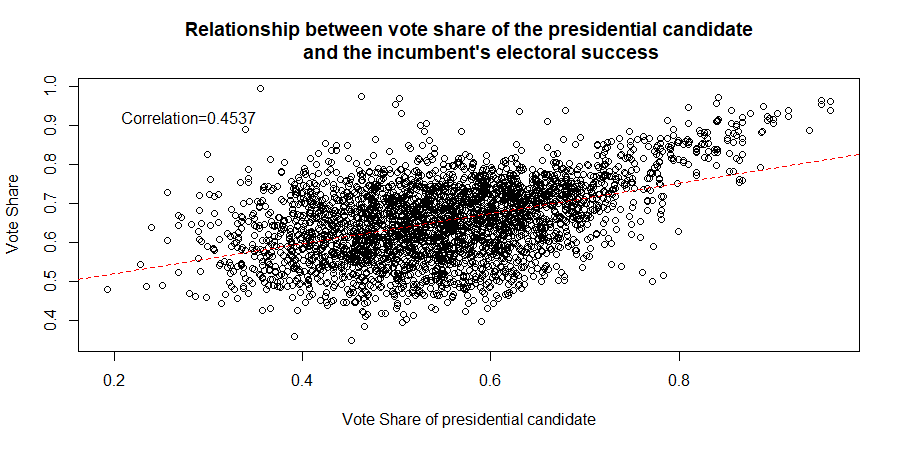
\includegraphics[width=1.3\textwidth]{Q3PS3.png}
    \caption{Relationship between vote share of the presidential candidate
     and the incumbent's electoral success}
    \label{}
\end{figure}
On the basis of the regression line and correlation value in Figure 3, we can say that there is a moderate positive correlation (0.4537) between vote share of presidential candidate and the vote share of the incumbent party.

\subsection{Answer 3c)}
The prediction equation for our simple linear regression is:

\begin{math}
    Vote Share = 0.441 + 0.388 * presvote 
\end{math}

\section{Question 4}
\subsection{Answer 4a)}
I run a linear regression using the lm function where the outcome variable is the residuals from question 1 and the explanatory variable is the residuals from question 2
\begin{verbatim}
    q4 <- lm(q1$residuals~q2$residuals)
    summary(q4)
\end{verbatim}

Our null hypothesis is that there is no association between the residuals from Q2 (X) and the Residuals from Q1 (Y), $\beta_1 = 0$

The alternative hypothesis is that there is an association between the residuals of Q2 (X) and the residuals of Q1 (Y), $\beta_1 \neq 0$

\begin{table}[!htbp] \centering 
  \caption{Bivariate regression between Q2-Residuals (X) and Q1-Residuals(Y)} 
  \label{} 
\begin{tabular}{@{\extracolsep{5pt}}lc} 
\\[-1.8ex]\hline 
\hline \\[-1.8ex] 
 & \multicolumn{1}{c}{\textit{Dependent variable:}} \\ 
\cline{2-2} 
\\[-1.8ex] & Q1-Residuals \\ 
\hline \\[-1.8ex] 
  Constant & $-$5.934e-18 \\ 
  & (0.001) \\ 
  & \\ 
  Q2-Residuals & 0.257$^{***}$ \\ 
  & (0.012) \\ 
  & \\ 
\hline \\[-1.8ex] 
Observations & 3,193 \\ 
R$^{2}$ & 0.130 \\ 
Adjusted R$^{2}$ & 0.130 \\ 
Residual Std. Error & 0.073 (df = 3191) \\ 
F Statistic & 476.975$^{***}$ (df = 1; 3191) \\ 
\hline 
\hline \\[-1.8ex] 
\textit{Note:}  & \multicolumn{1}{r}{$^{*}$p$<$0.1; $^{**}$p$<$0.05; $^{***}$p$<$0.01} \\ 
\end{tabular} 
\end{table} 

As shown in Table 4, $\beta_1$ is significant at the 0.01 alpha level, hence we can reject the null hypothesis and we find support for the alternative hypothesis that there is an association between the residuals from Question 2 (X) and the residuals from Question 1 (Y), $\beta_1 \neq 0$. 
Moreover, we can say that for a 1 unit increase in the residuals from Q2 (X), there is a 0.257 increase in the residuals from Q1 (Y).

\subsection{Answer 4b)}

I make a scatterplot with both variables along with a regression line and the correlation value:
\begin{verbatim}
plot(q2$residuals,q1$residuals,main='Relationship between 
    Residuals from Q1 and Residuals from Q2',
     xlab='Q2-Residuals',ylab='Q1-Residuals')
abline(q4,col='red',lty='dashed')
cor(q1$residuals,q2$residuals)
text(-0.22, 0.22,sprintf("Correlation=%s", round(cor(q1$residuals,q2$residuals),4)))
\end{verbatim}

\begin{figure} [h!] %%Code to put figures in the pdf
    \centering
    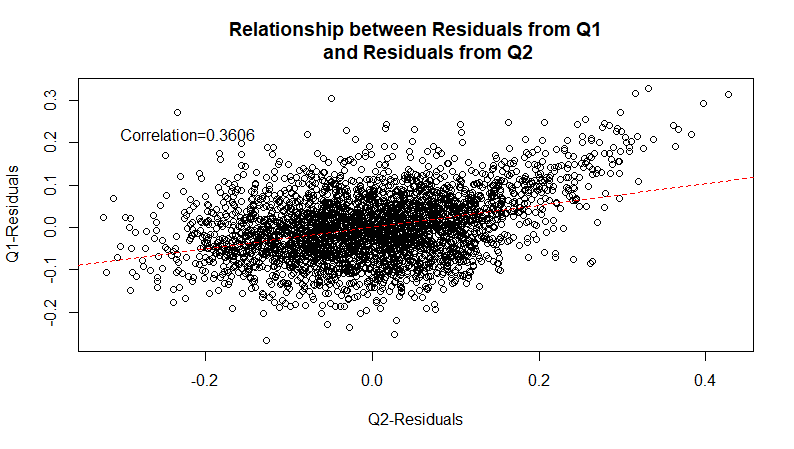
\includegraphics[width=1.3\textwidth]{Q4PS3.png}
    \caption{Relationship between Residuals from Q1 
    and Residuals from Q2}
    \label{}
\end{figure}
On the basis of the regression line and correlation value in Figure 4, we can say that there is a weak positive correlation (0.3606) between the residuals from Q1 and the residuals from Q2

\subsection{Answer 4c)}
The prediction equation for our simple linear regression is:

\begin{math}
    Q1Residuals = -5.934e-18 + 0.257 * Q2 Residuals 
\end{math}


\section{Question 5}
\subsection{Answer 5a}
I run a multiple linear regression using the lm function where the outcome variable is the incumbent's vote share and the explanatory variables are difflog and presvote

\begin{verbatim}
    q5 <- lm(voteshare~difflog+presvote, data=incumbent)
    summary(q5)
\end{verbatim}

For multiple linear regression, our null hypothesis for the F-test is that there is no relationship between the explanatory variables and the outcome variable, holding other variables constant, $\beta_i = 0$

The alternative hypothesis is that there is a relationship between the explanatory variables and the outcome variable, $\beta_i \neq 0$
\begin{table}[!htbp] \centering 
  \caption{Multiple linear regression model between difflog(X1),presvote(X2) and voteshare(Y)} 
  \label{} 
\begin{tabular}{@{\extracolsep{5pt}}lc} 
\\[-1.8ex]\hline 
\hline \\[-1.8ex] 
 & \multicolumn{1}{c}{\textit{Dependent variable:}} \\ 
\cline{2-2} 
\\[-1.8ex] & voteshare \\ 
\hline \\[-1.8ex] 
  Constant & 0.449$^{***}$ \\ 
  & (0.006) \\ 
  & \\ 
  difflog & 0.036$^{***}$ \\ 
  & (0.001) \\ 
  & \\ 
 presvote & 0.257$^{***}$ \\ 
  & (0.012) \\ 
  & \\ 
\hline \\[-1.8ex] 
Observations & 3,193 \\ 
R$^{2}$ & 0.450 \\ 
Adjusted R$^{2}$ & 0.449 \\ 
Residual Std. Error & 0.073 (df = 3190) \\ 
F Statistic & 1,302.947$^{***}$ (df = 2; 3190) \\ 
\hline 
\hline \\[-1.8ex] 
\textit{Note:}  & \multicolumn{1}{r}{$^{*}$p$<$0.1; $^{**}$p$<$0.05; $^{***}$p$<$0.01} \\ 
\end{tabular} 
\end{table} 

As we see in Table 5, the F statistic of 1,302.947 is significant at the 0.01 level and therefore, we can reject the null hypothesis and have support for the alternate hypothesis that at least one of the $\beta s \neq 0$.
This makes sense as both our individual regression coefficients for difflog and presvote are significant at the 0.01 level and hence, the F-test not being significant would be unusual. 

We can also interpret both the individual coefficients which are significant at the 0.01 level. 
First, we can say that for a 1 unit increase in difflog, this corresponds to a 0.036 scale points increase in vote share, while controlling for the effects of presvote 
Next, we can say that for a 1 unit increase in presvote, this corresponds to an increase of 0.257 scale points in vote share, while controlling for the effects of difflog.

\subsection{Answer 5b)}
The prediction equation for a multiple linear regression can be represented as:
\begin{math} \hat{Y} = \hat{\beta_0} + \hat{\beta_1} * X_1 + \hat{\beta_2} * X_2 + ... + \hat{\beta_p} * X_p \end{math} 

where:

\noindent $\hat{Y}$ is the predicted value of the outcome variable based on the multiple regression equation

\noindent $X_1, X_2,..,X_p$ are the explanatory variables

\noindent $\hat{\beta_0}$ is the estimated y-intercept or the constant term. This is the value of the outcome variable when all the explanatory variables are equal to zero

\noindent $\hat{\beta_1},\hat{\beta_2,...,\hat{\beta_p}}$ are the estimated coefficients corresponding to each explanatory variable

\noindent The error term, $\epsilon$ is inherent in the statistical model, but is not explicitly included in the prediction equation.

\vspace{0.3cm}

\noindent On the basis of this, the prediction equation for our multiple linear regression model is:

\begin{math}
    Vote Share = 0.449 + 0.036 * difflog + 0.257 * pres vote 
\end{math}

\subsection{Answer 5c)}
Question: What is it in this output that is identical to the output in Question 4? Why do you think this is the case?
\vspace{0.2cm}

Answer: \linebreak
The slope/regression coefficient for pres vote (0.257) in Question 5 is identical to the regression coefficient for Q2 residuals (0.257) in Question 4. Even their standard errors are the same.

This is my explanation for this phenomenon.
In Question 1, I looked at the relationship between difflog and vote share. The residuals for Question 1 represents the part of vote share that is not linearly related to difflog.
Simiarly, in Question 2, I looked at the relationship between difflog and pres vote. In this case, the residuals represent the part of pres vote that is not linearly related to difflog. 
Therefore, the regression coefficient in Question 4 between the residuals of Question 1 and Question 2 represents the effect of Pres vote on vote share after taking out the effects of difflog from both vote share and presvote. 
When it comes to multiple linear regression in Question 5, the regression coefficient (0.257) is the partial regression coefficient as it represents the contribution of presvote to the outcome variable of vote share after both variables had been linearly adjusted to the other predictor variable, difflog.
From this, we also learn that simple and multiple linear regression coefficients are not the same unless the explanatory variables are uncorrelated. When dealing with observational data, explanatory variables are rarely uncorrelated. Finally, this also helps in emphasizing the importance of controlling for other explanatory variables through multiple linear regression to better understand the relationship between different variables.

\end{document}
